%
% $RCSfile: translator_architecture.tex,v $
%
% Copyright (C) 2002-2008. Christian Heller.
%
% Permission is granted to copy, distribute and/or modify this document
% under the terms of the GNU Free Documentation License, Version 1.1 or
% any later version published by the Free Software Foundation; with no
% Invariant Sections, with no Front-Cover Texts and with no Back-Cover
% Texts. A copy of the license is included in the section entitled
% "GNU Free Documentation License".
%
% http://www.cybop.net
% - Cybernetics Oriented Programming -
%
% http://www.resmedicinae.org
% - Information in Medicine -
%
% Version: $Revision: 1.1 $ $Date: 2008-08-19 20:41:09 $ $Author: christian $
% Authors: Christian Heller <christian.heller@tuxtax.de>
%

\section{Translator Architecture}
\label{translator_architecture_heading}
\index{Translator Architecture}

Section \ref{a_changing_world_heading} emphasised the different roles of state-
and logic knowledge within systems and communication processes. This section
investigates how classical software system design handles both kinds of
knowledge models.

%
% $RCSfile: interacting_systems.tex,v $
%
% Copyright (C) 2002-2008. Christian Heller.
%
% Permission is granted to copy, distribute and/or modify this document
% under the terms of the GNU Free Documentation License, Version 1.1 or
% any later version published by the Free Software Foundation; with no
% Invariant Sections, with no Front-Cover Texts and with no Back-Cover
% Texts. A copy of the license is included in the section entitled
% "GNU Free Documentation License".
%
% http://www.cybop.net
% - Cybernetics Oriented Programming -
%
% http://www.resmedicinae.org
% - Information in Medicine -
%
% Version: $Revision: 1.1 $ $Date: 2008-08-19 20:41:07 $ $Author: christian $
% Authors: Christian Heller <christian.heller@tuxtax.de>
%

\subsection{Interacting Systems}
\label{interacting_systems_heading}
\index{Interacting Systems}
\index{Information Technology Environment}
\index{IT Environment}
\index{Physical Architecture}
\index{Logical Architecture}
\index{Data Mapper}
\index{Data Transfer Object}
\index{DTO}
\index{Model View Controller}
\index{MVC}
\index{Communication Patterns}
\index{Conversion between Communication Models}
\index{Frontend Communication Model}
\index{Backend Communication Model}
\index{Remote Communication Model}
\index{Domain Communication Model}
\index{Persistence Layer}

Chapter \ref{physical_architecture_heading} introduced an example
\emph{Information Technology} (IT) environment (\emph{Physical Architecture}),
containing many interacting systems: server and client, local and remote, human
and artificial (figure \ref{communication_figure}). In (object oriented)
software design, special patterns are used to architect a system such that it
is able to communicate with other systems across various mechanisms
(\emph{Logical Architecture}). To these patterns count the \emph{Data Mapper},
\emph{Data Transfer Object} (DTO) and \emph{Model View Controller} (MVC)
(section \ref{pattern_heading}).

\begin{figure}[ht]
    \begin{center}
        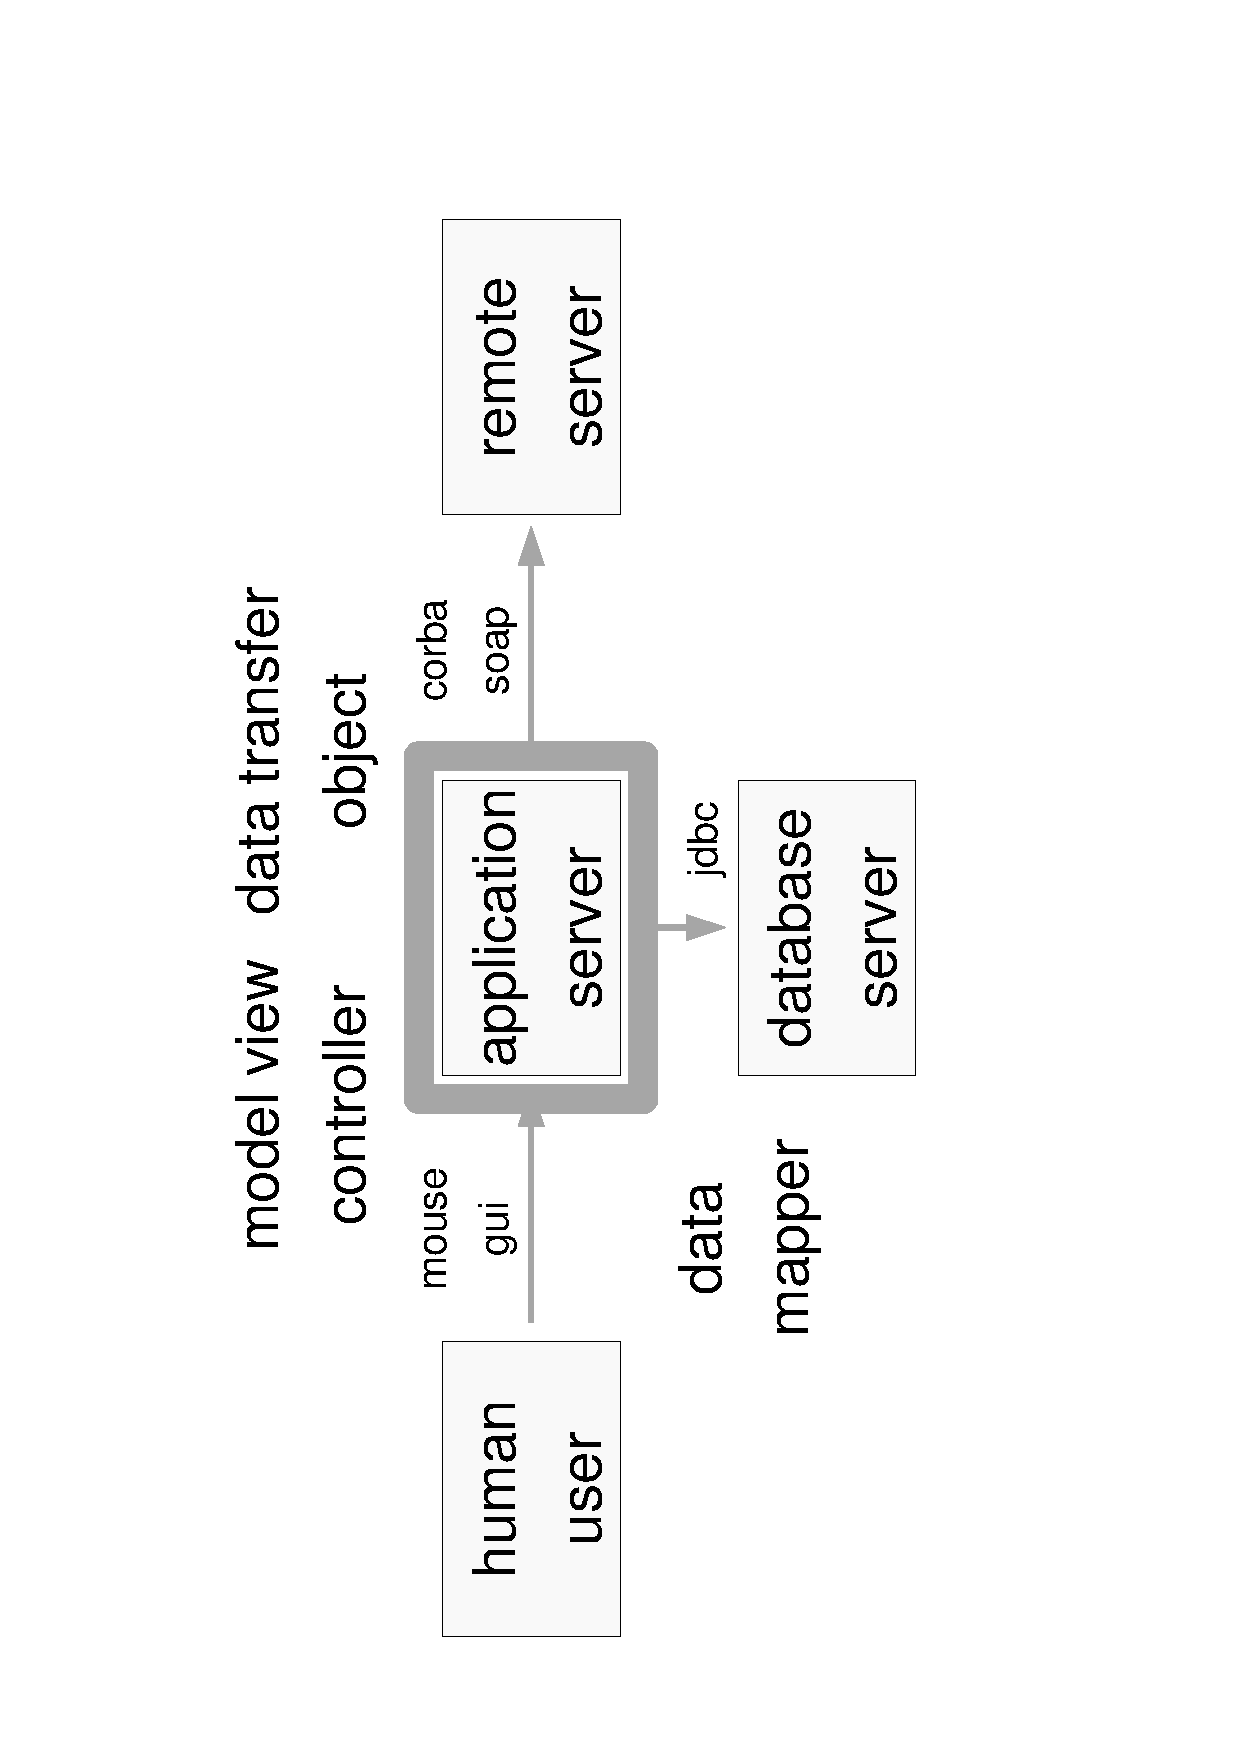
\includegraphics[scale=0.3,angle=-90]{graphic/communication.pdf}
        \caption{IT Environment with Server using Communication Patterns}
        \label{communication_figure}
    \end{center}
\end{figure}

Although software development has become a lot easier in the last decades, it is
still a big effort that should not be underestimated. One thing that application
developers have to care about much of their time is the \emph{Conversion}
between various kinds of (communication) models that a system has:

\begin{itemize}
    \item[-] Frontend (Communication with Human User)
    \item[-] Backend (Communication with Data Source)
    \item[-] Remote (Communication with Server)
    \item[-] Domain (Communication with own Knowledge)
\end{itemize}

The different mechanisms and patterns that have to be considered for such model
conversion often need to be implemented repeatedly, for each new application.
Some trials to unify all backend communication in a common \emph{Persistence Layer}
exist \cite{ambler}, but are remote- and frontend communication seldom considered
in a comparable way. Obviously, no current effort treats the frontend as just
another communication model that has to be \emph{sent} to the human user as
just another system.

The following sections will first reconsider three common communication
patterns, before embedding them into the classical model of logical system
layers (section \ref{layers_heading}). After that, a simplification is
suggested which finally leads to a new \emph{Translator Architecture} (first
introduced in \cite{hellerkunze}).

%
% $RCSfile: basic_patterns.tex,v $
%
% Copyright (c) 2001-2004. Christian Heller. All rights reserved.
%
% No copying, altering, distribution or any other actions concerning this
% document, except after explicit permission by the author!
% At some later point in time, this document is planned to be put under
% the GNU FDL license. For now, _everything_ is _restricted_ by the author.
%
% http://www.cybop.net
% - Cybernetics Oriented Programming -
%
% http://www.resmedicinae.org
% - Information in Medicine -
%
% @author Christian Heller <christian.heller@tuxtax.de>
%

\section{Basic Patterns}
\label{basic_patterns_heading}

%
% $RCSfile: data_mapper.tex,v $
%
% Copyright (c) 2004. Christian Heller. All rights reserved.
%
% No copying, altering, distribution or any other actions concerning this
% document, except after explicit permission by the author!
% At some later point in time, this document is planned to be put under
% the GNU FDL license. For now, _everything_ is _restricted_ by the author.
%
% http://www.cybop.net
% - Cybernetics Oriented Programming -
%
% http://www.resmedicinae.org
% - Information in Medicine -
%
% @author Christian Heller <christian.heller@tuxtax.de>
%

\paragraph{Data Mapper}
\label{data_mapper_heading}

Besides the \emph{Domain Logic}, standard three-tier architectures contain a
\emph{Data Source} layer which may for example represent a database. Both layers
need to exchange data. Modern systems use OOP methods to implement the domain
model. Database models, on the other hand, are often implemented as
\emph{Entity Relationship Model} (ERM).

In order to avoid close coupling and a mix-up of both layers, the introduction
of an additional \emph{Data Mapper} layer \cite{fowler2002} in between the two
others may be justified (figure \ref{datamapper_figure}). The most important
idea of this pattern is to abolish the interdependencies of domain- and
persistence model (database).

\begin{figure}[ht]
    \begin{center}
        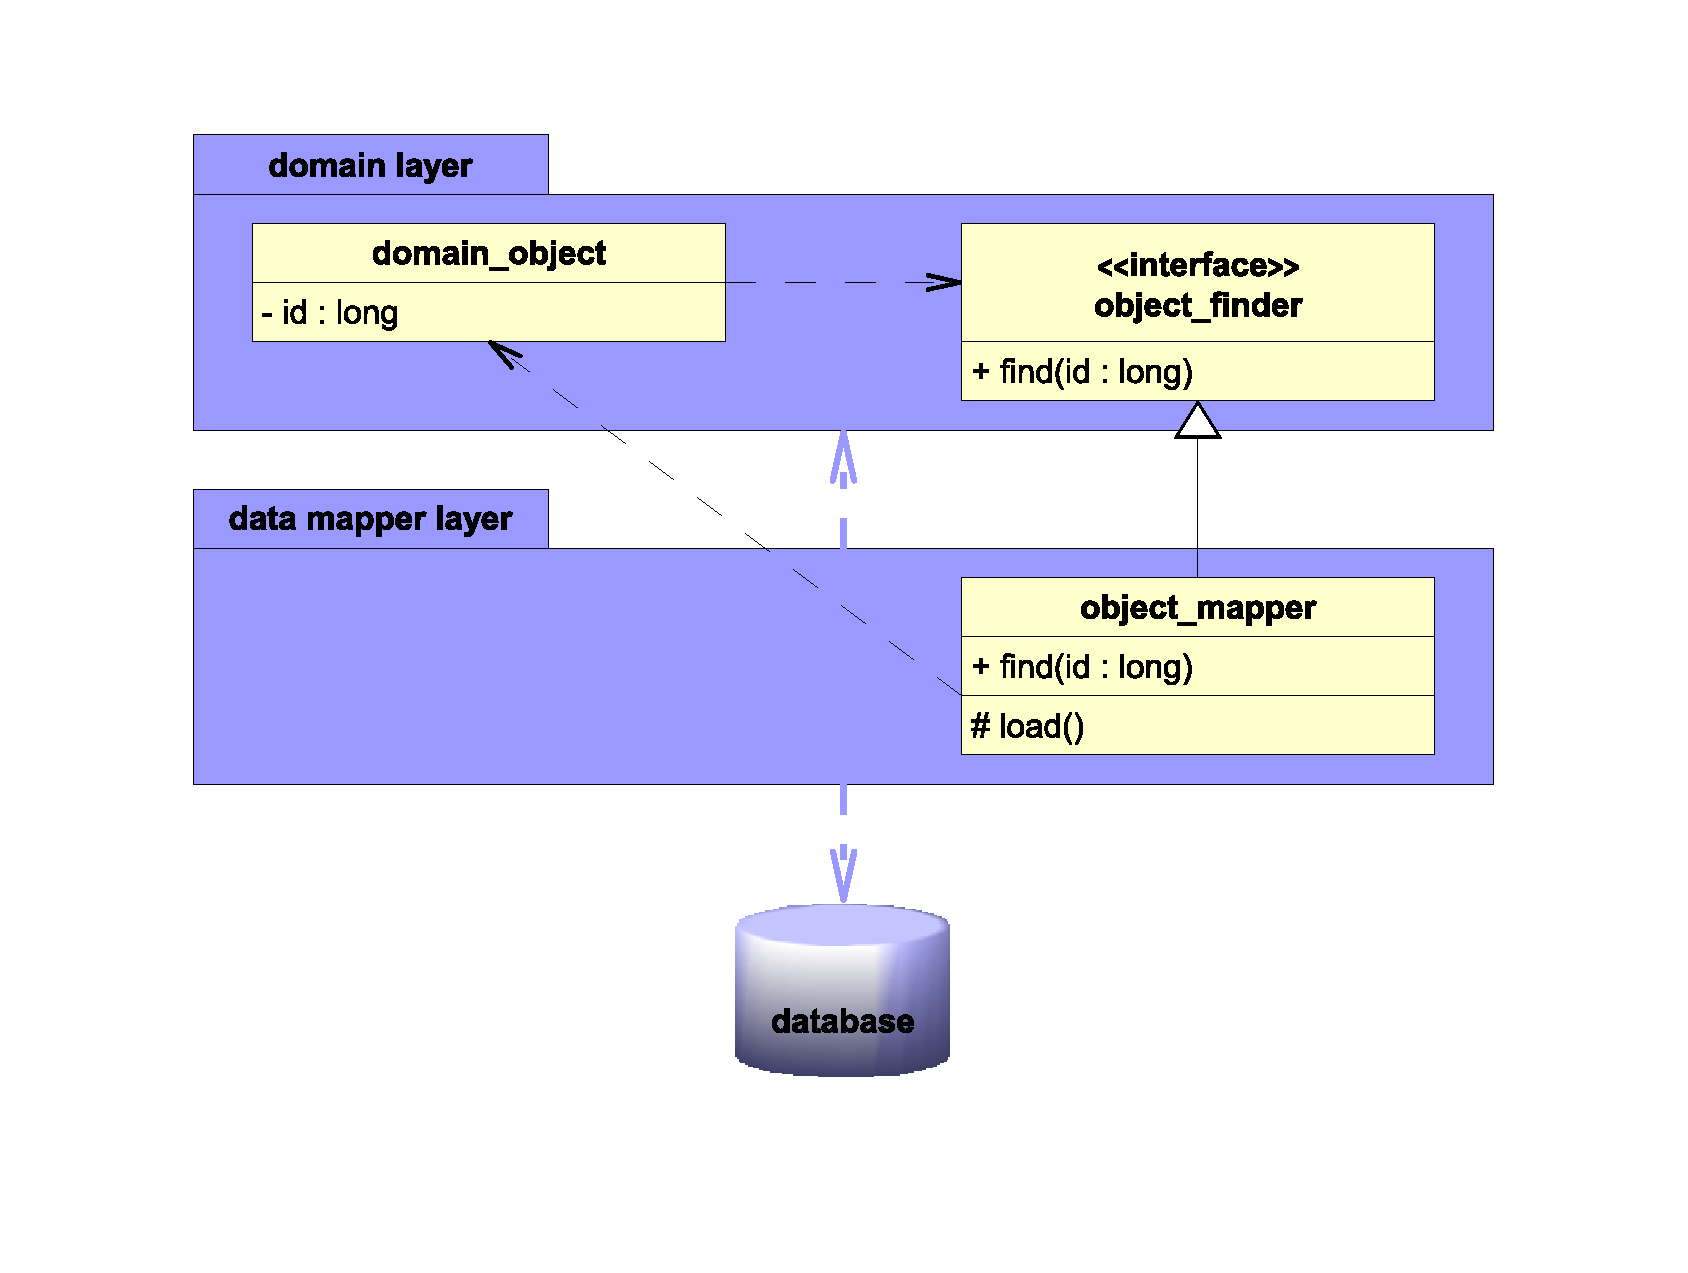
\includegraphics[scale=0.3]{vector/datamapper.eps}
        \caption{Data Mapper Pattern}
        \label{datamapper_figure}
    \end{center}
\end{figure}

The dashed arrows in figure \ref{datamapper_figure} indicate dependencies. The
data mapper layer knows the domain model- as well as the data source layer, via
\emph{unidirectional} relations. Its task is to \emph{translate} between the two,
in both directions. Domain model and data source know nothing from each other.

Each domain model class knows its appropriate interface (\emph{object\_finder})
but does not know the implementation of the same. That is, persistence- and
data retrieval mechanisms are hidden in front of the domain model. The
implementation (\emph{object\_mapper}) is part of the mapping package and also
implements all finder methods. It maps data of the received result sets to the
special attributes of the domain model objects.

The \emph{Mediator} pattern \cite{gamma1995} is similar to the \emph{Mapper}, in
that it is used to decouple different parts of a system. Fowler \cite{fowler2002}
writes: \textit{\ldots the objects that use a mediator are aware of it, even if
they aren't aware of each other; the objects that a mapper separates aren't even
aware of the mapper.}

Although the \emph{Data Mapper} pattern is very helpful at implementing OO
systems, two things are to be criticised:

Firstly, since the \emph{object\_finder} relies on functionality specific to the
retrieval of persistent data, it does actually belong into the data mapper layer
what, if done, would create bidirectional dependencies between the domain model-
and data mapper layer. But also with the \emph{object\_finder} remaining in the
domain model layer, dependencies are not purely unidirectional. It is true that
from an OO view, they are. Internally, however, a super class or interface
relates to its inheriting classes, so that it can call their methods to satisfy
the polymorphic behaviour.

Secondly, the layers do not truely build on each other. Taken a standard
architecture consisting of the following five -- instead of only three -- layers:

\begin{enumerate}
    \item Presentation
    \item Application Process
    \item Domain Model
    \item Data Mapper
    \item Data Source
\end{enumerate}

\ldots the application process does not only access the domain model layer, it
also has to manage (create and destroy) the objects of the data mapper layer.
In other words, it surpasses (disregards) the domain model layer when accessing
the data mapper layer directly.

%
% $RCSfile: data_transfer_object.tex,v $
%
% Copyright (C) 2002-2008. Christian Heller.
%
% Permission is granted to copy, distribute and/or modify this document
% under the terms of the GNU Free Documentation License, Version 1.1 or
% any later version published by the Free Software Foundation; with no
% Invariant Sections, with no Front-Cover Texts and with no Back-Cover
% Texts. A copy of the license is included in the section entitled
% "GNU Free Documentation License".
%
% http://www.cybop.net
% - Cybernetics Oriented Programming -
%
% http://www.resmedicinae.org
% - Information in Medicine -
%
% Version: $Revision: 1.1 $ $Date: 2008-08-19 20:41:06 $ $Author: christian $
% Authors: Christian Heller <christian.heller@tuxtax.de>
%

\subsubsection{Data Transfer Object}
\label{data_transfer_object_heading}
\index{Data Transfer Object Pattern}
\index{DTO}
\index{Assembler Object}
\index{Flat Data Structure}
\index{Translator Architecture}

\begin{figure}[ht]
    \begin{center}
       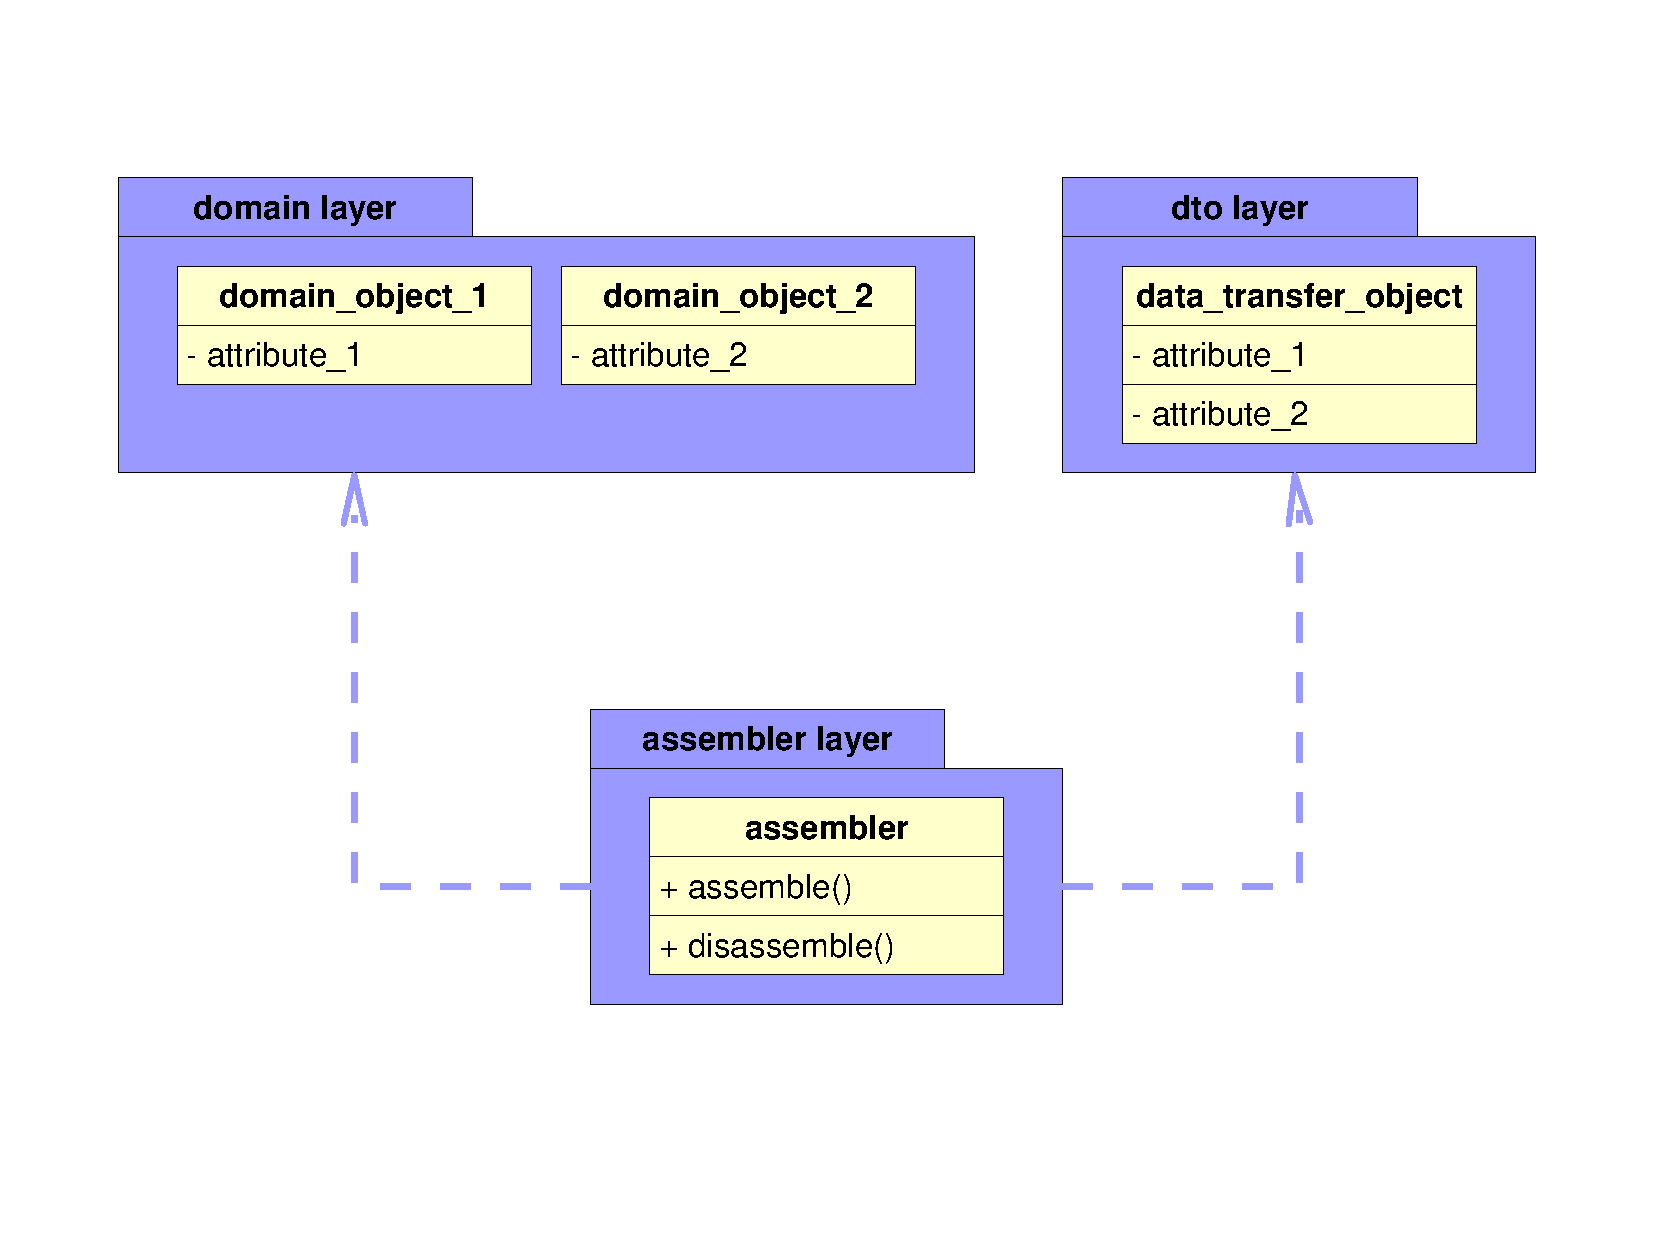
\includegraphics[scale=0.3,angle=-90]{graphic/dto.pdf}
       \caption{Data Transfer Object Pattern}
       \label{dto_figure}
    \end{center}
\end{figure}

It is a well-known fact that many small requests between two processes, and
even more between two hosts in a network need a lot of time. A local machine
with two processes has to permanently change the \emph{Program Context}; a
network has a lot of \emph{Transfers}. For each request, there is a necessity
of at least \emph{two} transfers -- the \emph{Question} of the client and the
\emph{Answer} of the server. Transfer methods are often expected to deliver
common data such as a Person's address, that is surname, first name, street,
zip-code, town and so on. These information is best retrieved by only
\emph{one} transfer call. That way, the client has to wait only once for a
server response and the server does not get too many single tasks. All address
data (in this example) would best be packaged together and sent back to the
client.

A scenario of that kind is exactly what the \emph{Data Transfer Object} pattern
\cite{fowler2002} proposes a solution for: A central \emph{Assembler} object
takes all common data of the server's domain model objects and assembles them
together into a special \emph{Data Transfer Object} (DTO), which is a flat data
structure (figure \ref{dto_figure}). The server will then send this DTO over
network to the client. On the client's side, a similar assembler takes the DTO,
finds out all received data and maps (disassembles) them to the client's domain
model. In that manner, a DTO is able to drastically improve the communication
performance.

Both, \emph{Data Mapper-} and DTO pattern translate one model into another. Due
to this similarity, chapter \ref{state_and_logic_heading} will try to merge
them into a common \emph{Translator} architecture.

%
% $RCSfile: model_view_controller.tex,v $
%
% Copyright (C) 2002-2008. Christian Heller.
%
% Permission is granted to copy, distribute and/or modify this document
% under the terms of the GNU Free Documentation License, Version 1.1 or
% any later version published by the Free Software Foundation; with no
% Invariant Sections, with no Front-Cover Texts and with no Back-Cover
% Texts. A copy of the license is included in the section entitled
% "GNU Free Documentation License".
%
% http://www.cybop.net
% - Cybernetics Oriented Programming -
%
% http://www.resmedicinae.org
% - Information in Medicine -
%
% Version: $Revision: 1.1 $ $Date: 2008-08-19 20:41:07 $ $Author: christian $
% Authors: Christian Heller <christian.heller@tuxtax.de>
%

\subsubsection{Model View Controller}
\label{model_view_controller_heading}
\index{Model View Controller Pattern}
\index{MVC}
\index{Graphical User Interface}
\index{GUI}
\index{Observer Pattern}
\index{Strategy Pattern}
\index{Wrapper Pattern}
\index{Composite Pattern}
\index{Java Foundation Classes}
\index{JFC}
\index{Microsoft Foundation Classes}
\index{MFC}
\index{Document View MVC Variant}
\index{Translator Architecture}

After having had a closer look at design patterns for persistence
(\emph{Data Mapper}) and communication (\emph{Data Transfer Object}), this
section considers the presentation layer of an application (figure
\ref{logical_figure}), which is often realised in form of a
\emph{Graphical User Interface} (GUI). Nowadays, the well-known
\emph{Model View Controller} (MVC) pattern \cite{buschmann, fowler2002} is used
by a majority of standard business applications. Its principle is to have the
\emph{Model} holding domain data, the \emph{View} accessing and displaying
these data and the \emph{Controller} providing the workflow of the application
by handling any action events happening on the view (figure \ref{mvc_figure}).
This separation eases the creation of applications with many synchronous views
on the same data. Internally, the MVC may consist of design patterns like:

\begin{figure}[ht]
    \begin{center}
        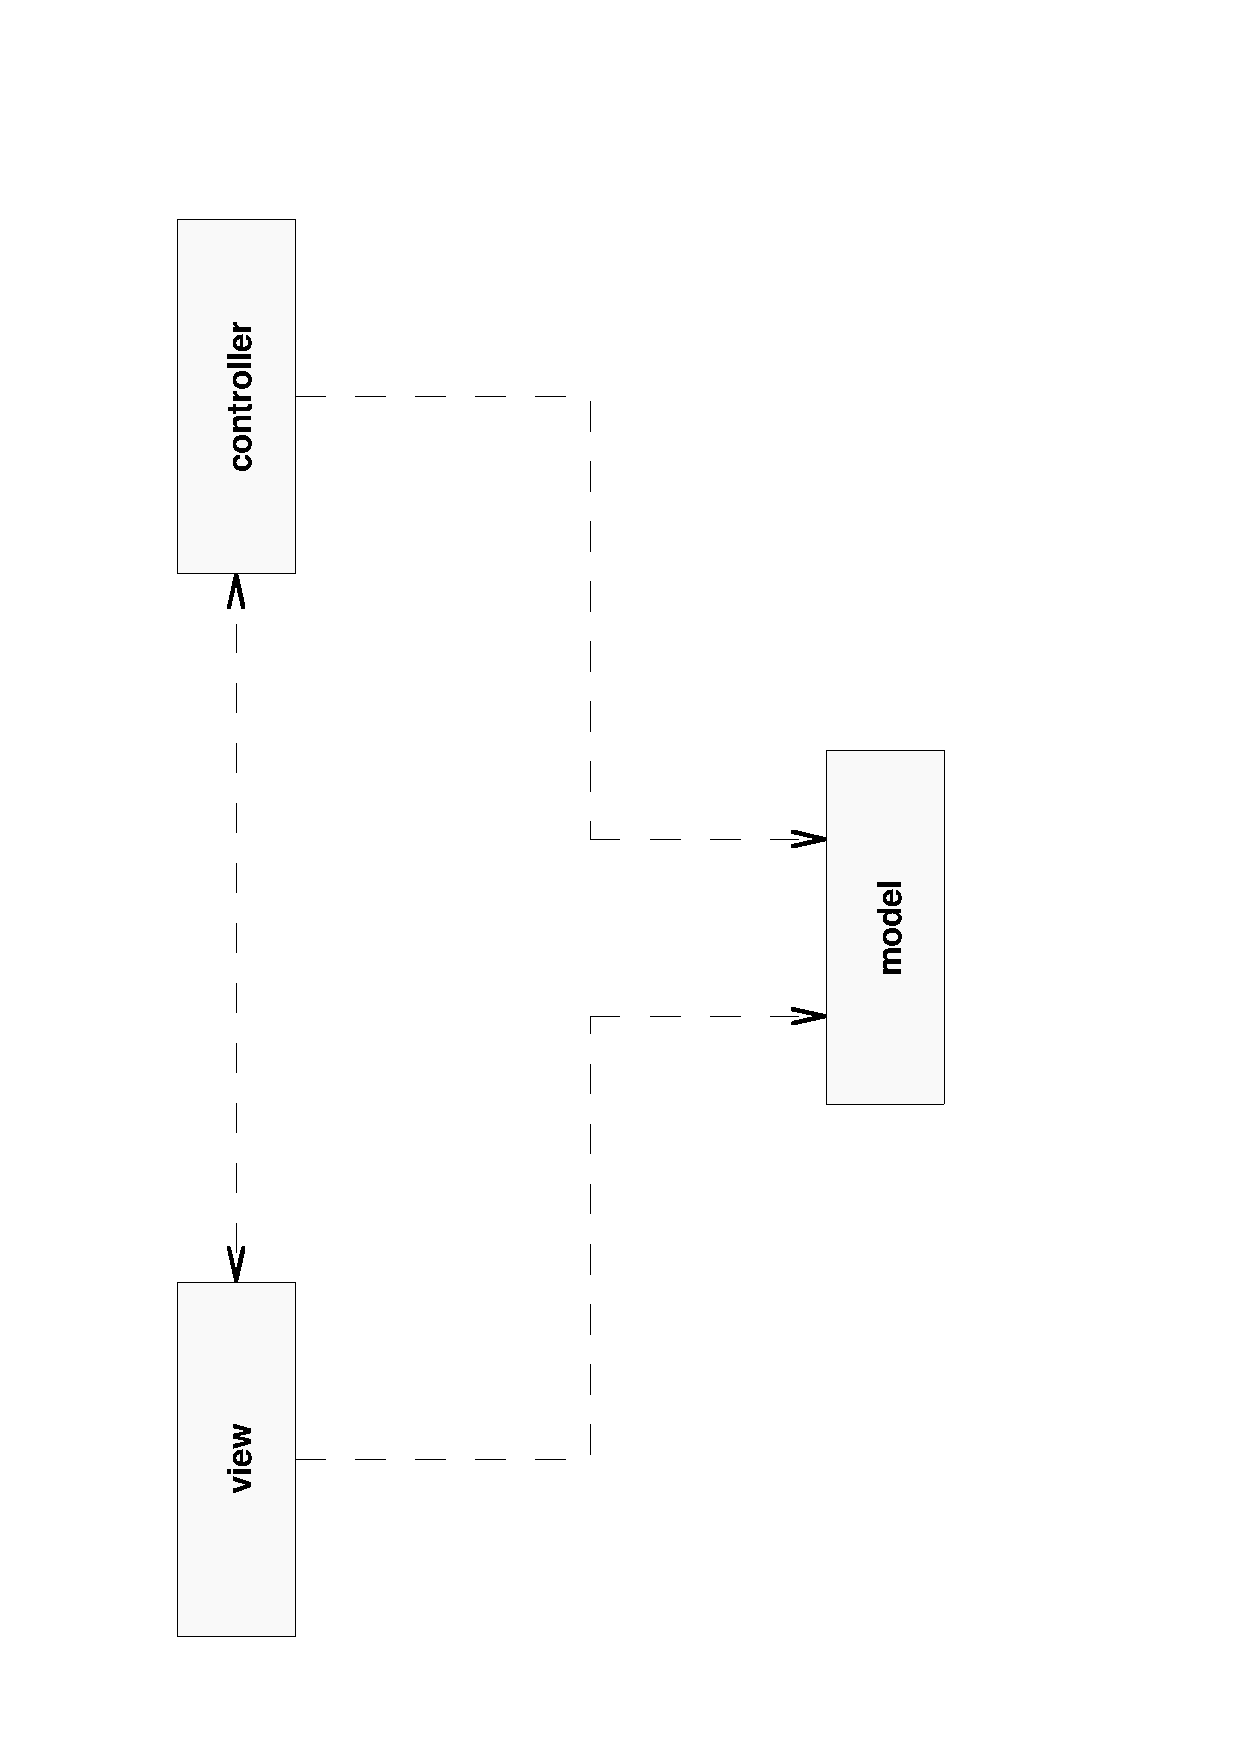
\includegraphics[scale=0.3,angle=-90]{graphic/mvc.pdf}
        \caption{Model View Controller Pattern}
        \label{mvc_figure}
    \end{center}
\end{figure}

\begin{itemize}
    \item[-] \emph{Observer} (section \ref{observer_heading}) which notifies
        the views about data model changes
    \item[-] \emph{Strategy} \cite{gamma1995} which encapsulates exchangeable
        functionality of the controller
    \item[-] \emph{Wrapper} (section \ref{wrapper_heading}) which delegates
        controller functionality to the \emph{Strategy}
    \item[-] \emph{Composite} (section \ref{composite_heading}) which equips
        graphical views with a hierarchical structure
\end{itemize}

Some MVC implementations like parts of the \emph{Java Foundation Classes} (JFC)
use a simplified version not separating controllers from their views. The
\emph{Microsoft Foundation Classes} (MFC) C++ library calls its implementation
\emph{Document-View}.

Besides the above-mentioned patterns \emph{Data Mapper} and DTO, MVC is the
third one getting merged into a common \emph{Translator} architecture, in
chapter \ref{state_and_logic_heading}.



%
% $RCSfile: placement.tex,v $
%
% Copyright (C) 2002-2008. Christian Heller.
%
% Permission is granted to copy, distribute and/or modify this document
% under the terms of the GNU Free Documentation License, Version 1.1 or
% any later version published by the Free Software Foundation; with no
% Invariant Sections, with no Front-Cover Texts and with no Back-Cover
% Texts. A copy of the license is included in the section entitled
% "GNU Free Documentation License".
%
% http://www.cybop.net
% - Cybernetics Oriented Programming -
%
% http://www.resmedicinae.org
% - Information in Medicine -
%
% Version: $Revision: 1.1 $ $Date: 2008-08-19 20:41:08 $ $Author: christian $
% Authors: Christian Heller <christian.heller@tuxtax.de>
%

\subsection{Placement}
\label{placement_heading}
\index{Layered Architecture}
\index{Communication Patterns placed in Layered Architecture}
\index{Model View Controller Pattern}
\index{MVC}
\index{Presentation Layer}
\index{Data Mapper Pattern}
\index{Entity Relationship Model}
\index{ERM}
\index{Database}
\index{DB}
\index{Data Transfer Object}
\index{DTO}
\index{Assembler}

Many state-of-the-art software systems consist of a layered architecture
similar to the one shown in figure \ref{logical_figure}. Yet how do the
communication patterns explained before suit this classical architecture? In
the traditional model of a layered software system, a startable process, best
placed in the \emph{Controller}, creates the whole application tree, to which
belong the \emph{Views} (as user interface), several \emph{Models} of the
\emph{Domain} (providing data to the views and as facade to remote servers) and
the \emph{Data Mapper} (translating between domain- and database model).

\begin{figure}[ht]
    \begin{center}
        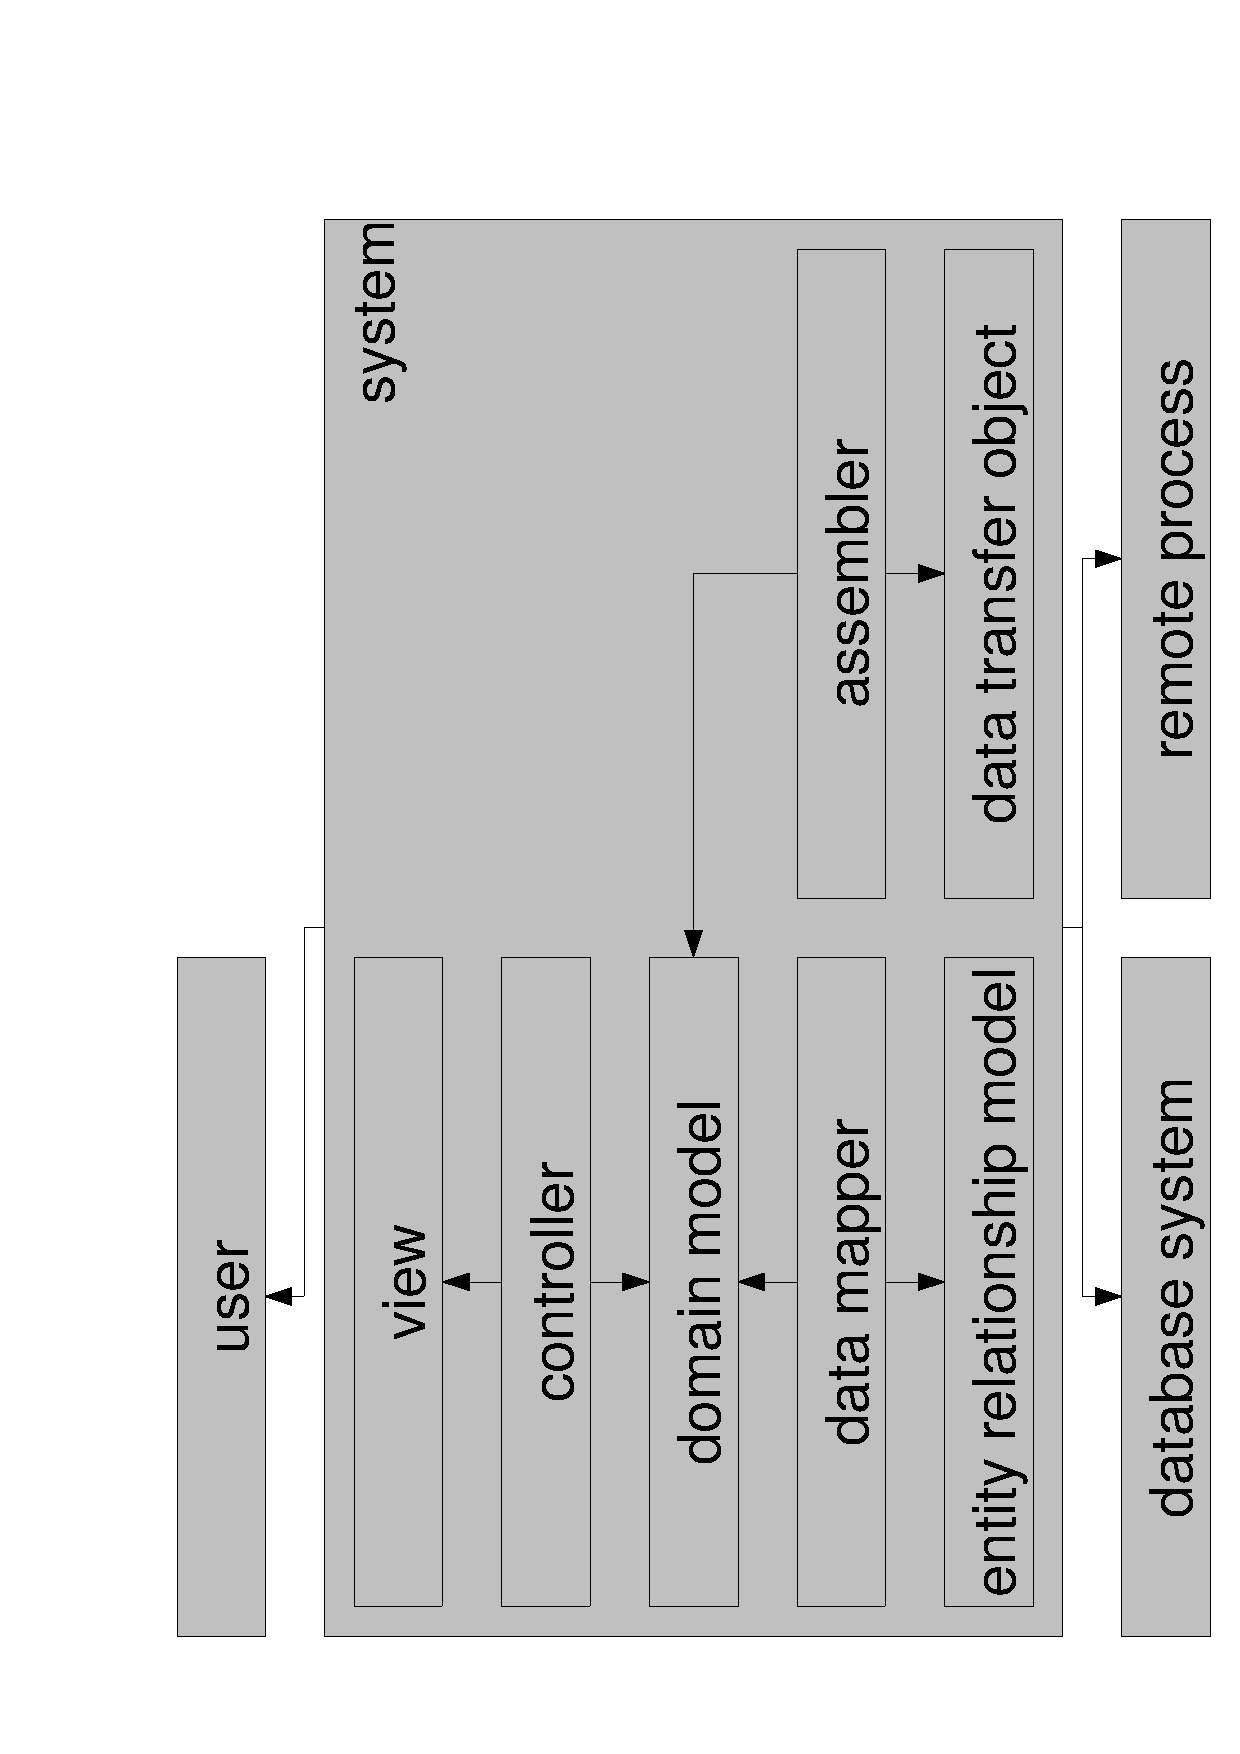
\includegraphics[scale=0.3,angle=-90]{graphic/placement.pdf}
        \caption{Communication Patterns placed in Layered Architecture}
        \label{placement_figure}
    \end{center}
\end{figure}

It is not difficult to figure out where the communication patterns of section
\ref{basic_patterns_heading} fit in here (figure \ref{placement_figure}): The
\emph{Model View Controller} (\emph{Presentation Layer}) determines the parts
to interact with a human user via the \emph{View}; the \emph{Data Mapper}
pattern with its inherent \emph{Entity Relationship Model} (ERM) encapsulates
mechanisms to connect to a persistence medium such as a \emph{Database} (DB);
the \emph{Data Transfer Object} (DTO) and its corresponding assemblers,
finally, serve as means of communication with remote servers.

%
% $RCSfile: simplification.tex,v $
%
% Copyright (C) 2002-2008. Christian Heller.
%
% Permission is granted to copy, distribute and/or modify this document
% under the terms of the GNU Free Documentation License, Version 1.1 or
% any later version published by the Free Software Foundation; with no
% Invariant Sections, with no Front-Cover Texts and with no Back-Cover
% Texts. A copy of the license is included in the section entitled
% "GNU Free Documentation License".
%
% http://www.cybop.net
% - Cybernetics Oriented Programming -
%
% http://www.resmedicinae.org
% - Information in Medicine -
%
% Version: $Revision: 1.1 $ $Date: 2008-08-19 20:41:08 $ $Author: christian $
% Authors: Christian Heller <christian.heller@tuxtax.de>
%

\subsection{Simplification}
\label{simplification_heading}
\index{System as Part of Communication}
\index{Model as Part of Communication}
\index{Translator as Part of Communication}
\index{Simplified Layered Architecture}
\index{State Knowledge}
\index{Logic Knowledge}

For all three kinds of communication, there is a:

\begin{itemize}
    \item[-] \emph{System} (Human User, Database, Remote Server)
    \item[-] \emph{Model} (View, ERM, DTO)
    \item[-] \emph{Translator} (Controller/ View Assembler, Data Mapper, DTO Assembler)
\end{itemize}

\begin{figure}[ht]
    \begin{center}
        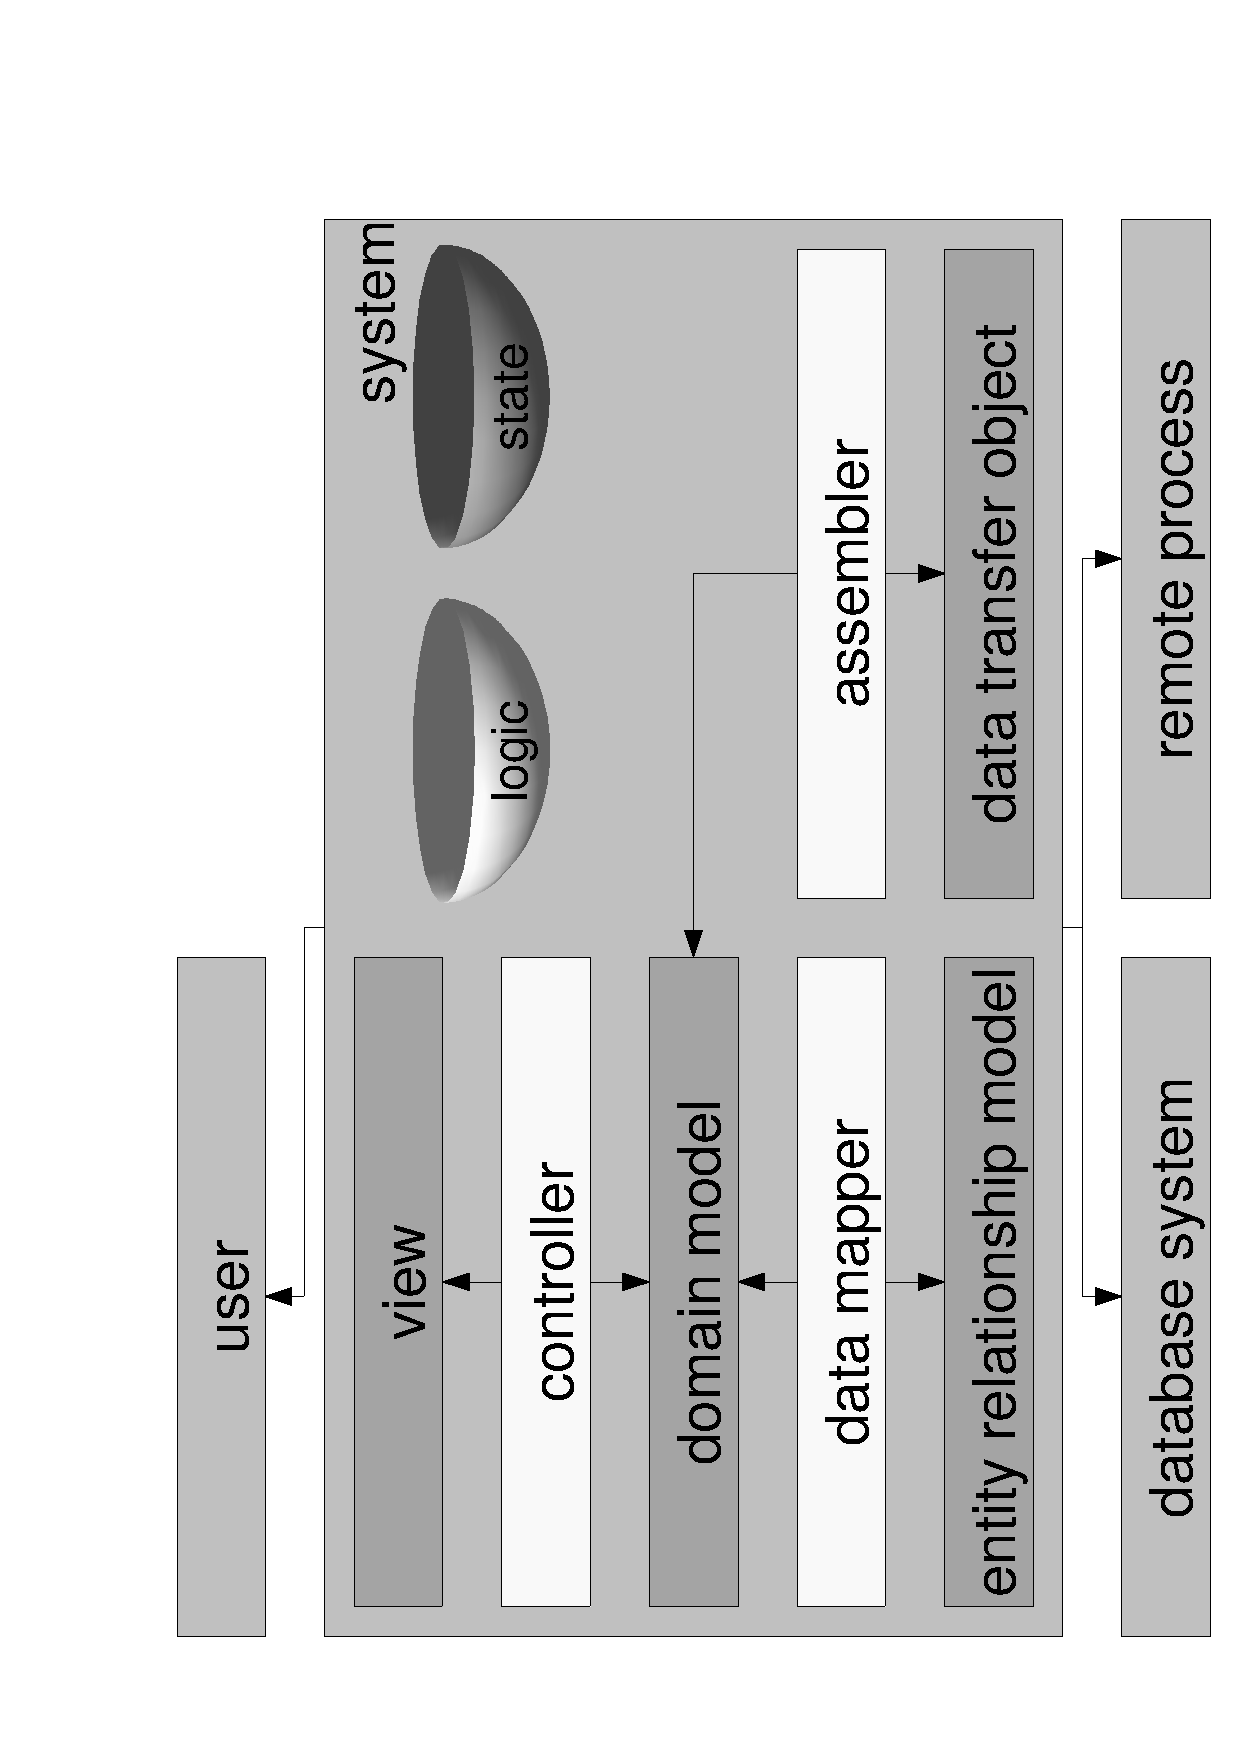
\includegraphics[scale=0.3,angle=-90]{graphic/simplification.pdf}
        \caption{Simplified Layered Architecture with State-/ Logic Knowledge}
        \label{simplification_figure}
    \end{center}
\end{figure}

All models represent certain states; all translators contain logic for
converting one state into another; all systems host their own, specific pool of
state- and logic knowledge. Realising this, a much clearer view on software
architectures can be retrieved (figure \ref{simplification_figure}).

Existing communication patterns can be merged into this common architecture.
Although these patterns suggest their very own communication paradigms, the
basic principles of interaction, as investigated on the example of transient
and persistent communication of humans in section \ref{communication_heading},
remain the same:

\begin{quote}
    An active \emph{System} (concrete process) has a mental state represented
    by passive \emph{Knowledge}. In order to exchange information with another
    system, it translates parts of its domain- into a special communication
    model which it sends to the other system. This is done by accessing its
    hardware infrastructure with \emph{input/ output} (i/o) abilities. The
    other system receives the communication model and translates it back to its
    own domain model.
\end{quote}

Because domain models differ between systems, each system needs its own
translator models. Only communication models need to be agreed upon between
systems; they need to be understood by both communication partners.

%
% $RCSfile: communication_model.tex,v $
%
% Copyright (C) 2002-2008. Christian Heller.
%
% Permission is granted to copy, distribute and/or modify this document
% under the terms of the GNU Free Documentation License, Version 1.1 or
% any later version published by the Free Software Foundation; with no
% Invariant Sections, with no Front-Cover Texts and with no Back-Cover
% Texts. A copy of the license is included in the section entitled
% "GNU Free Documentation License".
%
% http://www.cybop.net
% - Cybernetics Oriented Programming -
%
% http://www.resmedicinae.org
% - Information in Medicine -
%
% Version: $Revision: 1.1 $ $Date: 2008-08-19 20:41:05 $ $Author: christian $
% Authors: Christian Heller <christian.heller@tuxtax.de>
%

\subsection{Communication Model}
\label{communication_model_heading}
\index{Communication Model}
\index{Medium of Communication}
\index{Domain Model}
\index{Transfer Model}
\index{Model Translator}
\index{Mapping Rules}
\index{Notation}
\index{Rules of Translation}
\index{Textual User Interface}
\index{TUI}
\index{Graphical User Interface}
\index{GUI}
\index{Web User Interface}
\index{WUI}
\index{x Datentr\"ager}
\index{xDT}
\index{Healthcare Xchange Protocol}
\index{HXP}
\index{Clinical Document Architecture}
\index{CDA}

As section \ref{communication_heading} pointed out, systems (alive or not)
never communicate directly, but always across the detour of an external
(transient or persistent) \emph{Medium}. This makes it necessary to use special
\emph{Communication Models}, since nearly always, only \emph{parts} of a
complete \emph{Domain Model} want to be exchanged. The use of communication
(transfer) models again, entails the use of model \emph{Translators}. Sowa
\cite{sowa} writes in his book \emph{Knowledge Representation}:

\begin{quote}
    In computer science, there is no end to the number of specialized notations.
    Besides the hundreds of programming languages, there are diagrams for circuits,
    flowcharts, parse trees, game trees, Petri nets, PERT charts, neural networks,
    design languages, and novel notations that are invented whenever two
    programmers work out ideas at the blackboard. Musical notation \ldots\
    is an example of a complex language that is both precise and human factored.
    As long as the mapping rules are defined, all of these notations can be
    automatically translated to or from logic.
\end{quote}

\begin{figure}[ht]
    \begin{center}
        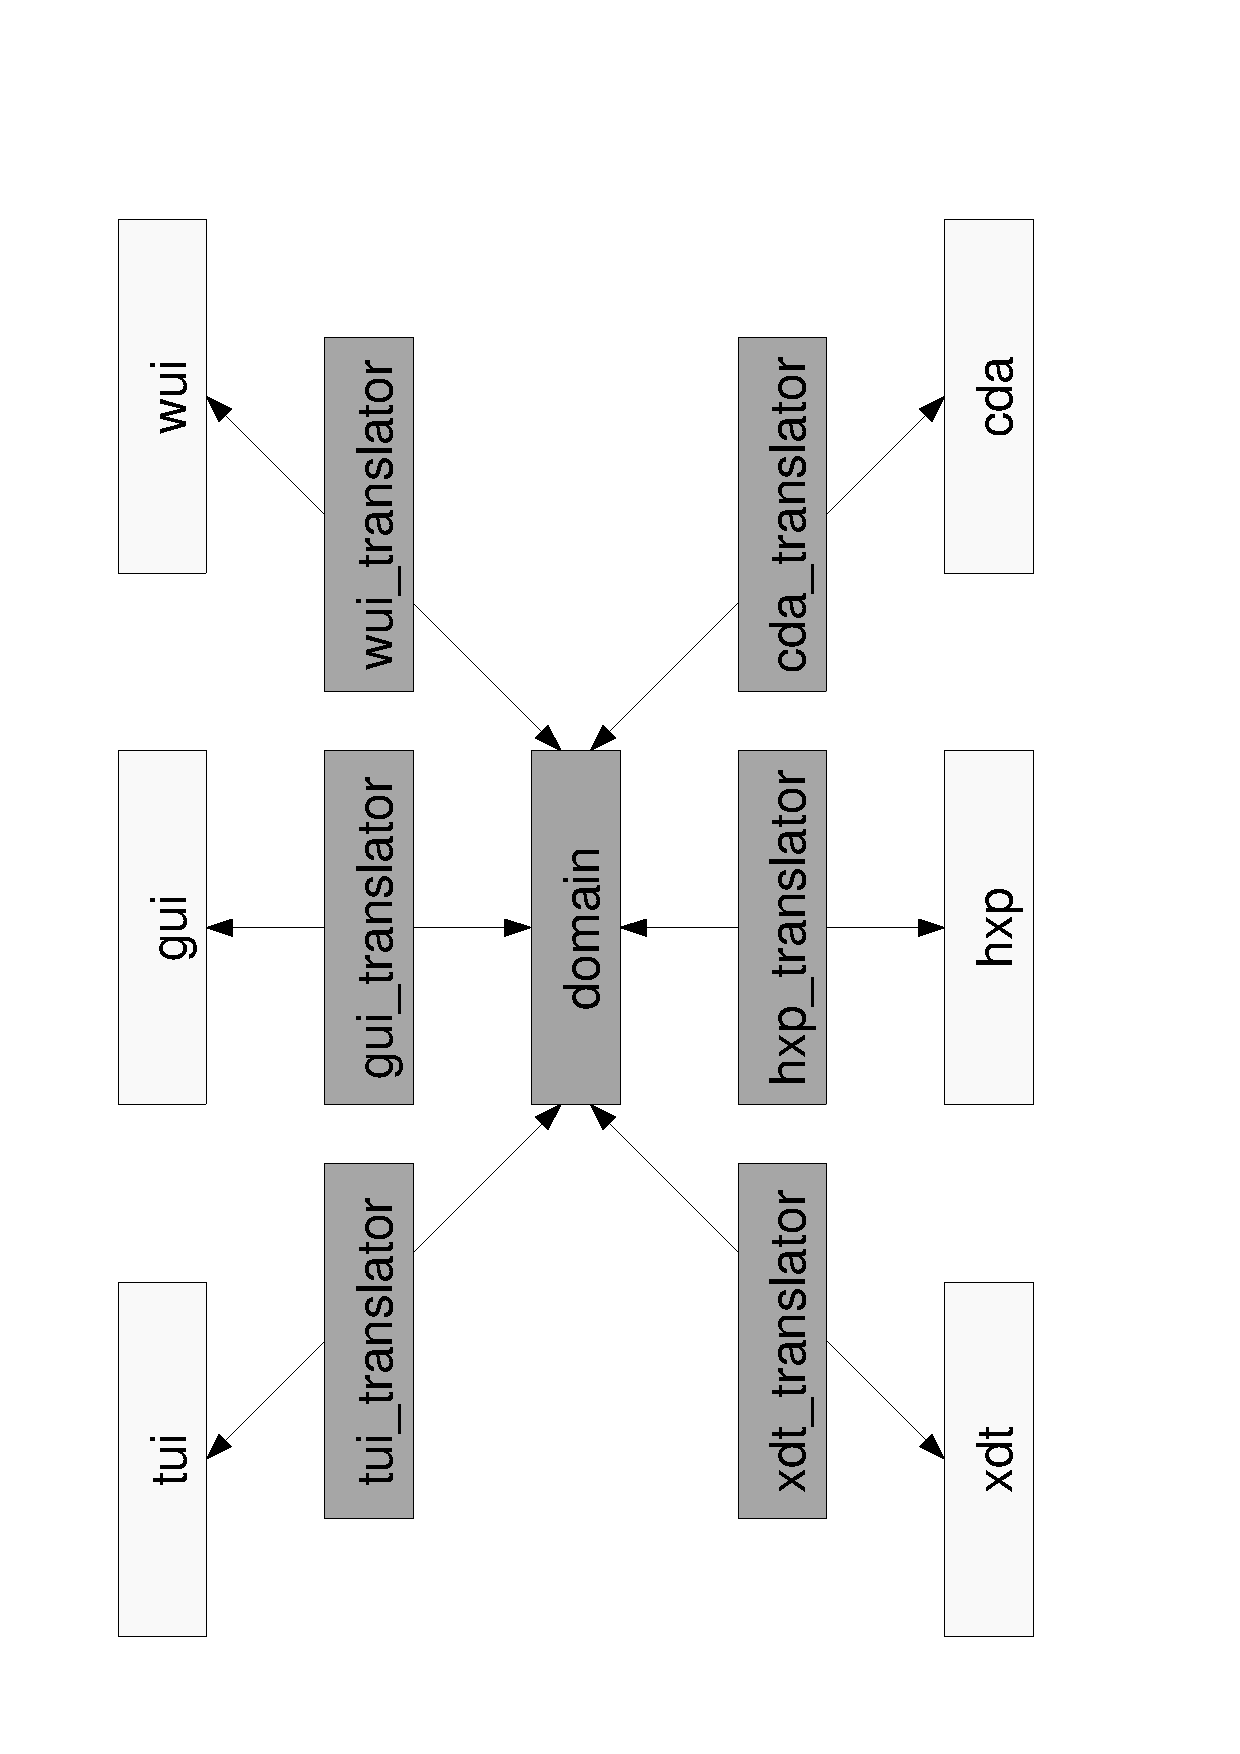
\includegraphics[scale=0.3,angle=-90]{graphic/translators.pdf}
        \caption{Different Kinds of Model Translators}
        \label{translators_figure}
    \end{center}
\end{figure}

Although he does not talk of \emph{Domain-} and \emph{Communication Models},
but of \emph{Notations}, Sowa obviously means the same: Any kind of abstract
model can be translated into any other kind, as long as the translation
\emph{Rules} are defined. Model \emph{Translators} are able to map domain model
data to transfer model data. Depending on which communication style is used,
different translators with different rules need to be applied.

Figure \ref{translators_figure} shows a number of possible model translators,
for a: \emph{Textual User Interface} (TUI), \emph{Graphical User Interface}
(GUI) and \emph{Web User Interface} (WUI) as well as for the German standard
file format for exchanging medical data called \emph{x Datentr\"ager} (xDT),
the \emph{Healthcare Xchange Protocol} (HXP) and HL7's exchange format called
\emph{Clinical Document Architecture} (CDA). More on these standards in chapter
\ref{res_medicinae_heading}.

Many application systems have exactly one domain model but transfer models of
arbitrary type should be addable anytime. Translators only know how to
translate between the domain model and a special transfer model, of course in
both directions. \emph{Direct} translation between transfer models is an
exception; it is possible but better done \emph{via} the domain model.

The type of transfer model is independent from the communication mechanism
used. The usage of a \emph{Graphical User Interface} (GUI) model, for example,
is not necessarily limited to human-computer interaction. It could very well be
used for data transfer between remote computers, as long as both systems know
how to translate that model.

%%
% $RCSfile: knowledge_split.tex,v $
%
% Copyright (C) 2002-2008. Christian Heller.
%
% Permission is granted to copy, distribute and/or modify this document
% under the terms of the GNU Free Documentation License, Version 1.1 or
% any later version published by the Free Software Foundation; with no
% Invariant Sections, with no Front-Cover Texts and with no Back-Cover
% Texts. A copy of the license is included in the section entitled
% "GNU Free Documentation License".
%
% http://www.cybop.net
% - Cybernetics Oriented Programming -
%
% http://www.resmedicinae.org
% - Information in Medicine -
%
% Version: $Revision: 1.1 $ $Date: 2008-08-19 20:41:07 $ $Author: christian $
% Authors: Christian Heller <christian.heller@tuxtax.de>
%

\subsection{Knowledge Split}
\label{knowledge_split_heading}

refer back to section \ref{input_output_and_rules_heading}

The \emph{Knowledge Query and Manipulation Language} (KQML) (section
\ref{knowledge_query_and_manipulation_language_heading}), a popular means of
communication in \emph{Agent Oriented Programming} (section
\ref{agent_oriented_programming_heading}), relies on \emph{Speech Act Theory}
developed by Searle 1960 and enhanced by Winograd and Flores in the 70s.
\cite{wikipedia} http://en.wikipedia.org/wiki/Agent\_communication\_language

- describe some language differences: CYBOL in comparison to Agent0:
http://www.cs.caltech.edu/~bond/courses/cs101c/agents16/node13.html
(states=believes, logic=capabilities, signal=commitment)
Do Agent0 and others provide the most suitable format to represent knowledge?

Two Comparison Tables:

1 with Agent0

http://www.cs.caltech.edu/~bond/courses/cs101c/agents16/node3.html

Mental State
    Beliefs (= Facts)
        ?? State Knowledge
    Commitments (to act, are grounded, that is do not contain variables)
        pre-defined actions are: DO, INFORM, REQUEST, UNREQUEST, REFRAIN, IF
        ?? Signal (signal removal is called "Release of a Commitment")
    Capabilities (= Actions; Commitments to oneself are special capabilities called Decision or Choice)
        ?? Logic Knowledge

Goals?
Intentions?
Time is treated as realtime; it is expressed explicitly, that is by adding it
to statements.
Action is represented by the fact that it happened at a given time;
since actions are facts they are also instantaneous.
Messages are passed by agents to each other, by message name.

2 with Kuehnel

- can all the different vocabulary (see Kuehnel: action, plan, assumption, aim/goal)
be simplified/unified into an easier system?
- Agents know about the environment and their own expertise
- add table for comparison between CYBOP and AGOP, for example:
    state knowledge = beliefs: capabilities (knowledge about itself)
        + constraints (knowledge about environment)
    logic knowledge = actions + plans
    signal = goal (aim)
- this is a comparison \emph{Trial} -- terms of AGOP are anyway not used uniformly in science

- ideas to split knowledge itself into state- and logic (action/ plan) knowledge
- see \cite[p. 95 ff., p. 125 ff.]{kuehnel}

%%
% $RCSfile: bundling.tex,v $
%
% Copyright (C) 2002-2008. Christian Heller.
%
% Permission is granted to copy, distribute and/or modify this document
% under the terms of the GNU Free Documentation License, Version 1.1 or
% any later version published by the Free Software Foundation; with no
% Invariant Sections, with no Front-Cover Texts and with no Back-Cover
% Texts. A copy of the license is included in the section entitled
% "GNU Free Documentation License".
%
% http://www.cybop.net
% - Cybernetics Oriented Programming -
%
% http://www.resmedicinae.org
% - Information in Medicine -
%
% Version: $Revision: 1.1 $ $Date: 2008-08-19 20:41:05 $ $Author: christian $
% Authors: Christian Heller <christian.heller@tuxtax.de>
%

\subsection{Bundling}
\label{bundling_heading}

OOP
\emph{Classes} as known from \emph{Object Oriented Programming} (OOP) bundle
attributes and methods which often causes additional inter-dependencies in a
system because classes do not only have to relate to other classes for accessing
their attributes but also for using the methods offered by them.

Bean/ Enterprise Java Bean (EJB)

- JMS Eigenschaften werden in EJBs eingebaut, so dass diese selbststaendig
andere EJBs aufrufen koennen.
- Verlagerung eines Teils der Application Logic into domain
--> bliebe nur noch 1 Schicht uebrig, die Domain (Gehirn)
--> Unguenstig, da mehrere verschiedene Sichten auf Domain gewuenscht und notwendig;
daher immer nur Domain-Extracts in Application dargestellt!
- How about adding a GUI to every EJB so that it can be displayed automatically?
--> useless: users want different guis and EJB data need to be displayed in
different contexts
==> the concept of merging more and more functionality into components a la EJB
is not arbitrarily continuable, nor always desired (different views on domain)

